\chapter{Resultados}
\label{cap:results}

\section{RQ1. Com que frequência \textit{breaking changes} impactam nos pacotes clientes?}

Nesta Seção, encontram-se os resultados da análise manual voltados para responder a primeira questão de pesquisa. Nessa Seção estão os dados relacionados à quantificação das \textit{breaking changes}.

\subsubsection{\textbf{10.4\% dos clientes e 8.4\% das \textit{releases} sofreram \textit{breaking changes}}}

De todos os 384 clientes que tiveram seus testes executados, 40 (10.4\%) apresentaram algum caso de \textit{breaking changes}. Entretanto, os clientes podem ser impactados por mais de um tipo de erro, por exemplo, uma \textit{release} pode ser impactada por uma \textit{breaking change} e outra, por um erro interno. Assim, o mesmo cliente pode ser classificado em dois, ou mais, tipos de erros. Por isso, os resultados são melhores apresentados em função das \textit{releases}, uma vez que uma \textit{release} só pode ser impactada por apenas um tipo de erro. Desta maneira, analisando as \textit{releases}, de todas as \textit{2300} que tiveram seus testes executados, 902 (39.5\%) sofreram algum tipo de erro, que foram:

\begin{itemize}
    \item 433 (18.7\%) das \textit{releases} foram impactadas por erros internos;
    \item os casos particulares de \textit{breaking changes} impactaram 213 (9.2\%) das \textit{releases};
    \item as \textit{breaking changes} impactaram 193 (8.4\%) \textit{releases}; e
    \item 73 (3.2\%) das \textit{releases} foram impactadas por algum erro que não foi descoberto.
\end{itemize}{}

A Tabela \ref{tab:pre_res_rq1} contém os resultados em função das \textit{releases}.

\begin{table}[]
\centering
\begin{tabular}{lr}
\toprule
\textbf{Resultados}                & \textbf{\%} \\ \hline
Sucesso                                & 60.5\%      \\
Erros internos                         & 18.7\%      \\
Casos particulares de \textit{breaking changes} & 9.2\%       \\
\textit{Breaking changes}              & 8.4\%       \\
Não encontrados                        & 3.2\%       \\ \bottomrule
\end{tabular}\caption{Resultado da análise em cada caso de erro}
\label{tab:pre_res_rq1}
\end{table}

\subsubsection{Relação das \textit{releases} do cliente com os provedores e as \textit{breaking changes}}

Após analisar todos os casos de testes que resultaram em erro, foram constatados um total de 40 (10.4\%) clientes impactados por \textit{breaking changes}. Esses clientes sofreram com \textit{breaking changes} em pelo menos uma de suas \textit{releases}. Desde clientes com os testes executados em apenas uma \textit{release}, até os clientes com mais de 100 \textit{releases} foram impactados e, de maneira análoga, clientes com 1 provedor até clientes com mais de 100 provedores também foram impactados por \textit{breaking changes}. Observando apenas a amostra, é possível verificar que há uma correlação entre o número de \textit{releases} e o número de provedores, conforme a Figura \ref{fig:correlation_release_providers} apresenta. Nessa Figura, cada ponto representa um cliente com sua determinada quantidade de provedores e de \textit{releases}, respectivamente nos eixos \textit{x} e \textit{y}, também há uma regressão não-linear que caracteriza a correlação entre a quantidade de provedores e a quantidade de \textit{releases} que tiveram os testes executados, e por fim, há uma linha vertical e uma horizontal significando a mediana das \textit{releases} e dos provedores da amostra, respectivamente, sendo que essas medianas valem 3 e 9, assim, dividindo o plano cartesiano em 4 quadrantes. \daniel{havia alguns outliers que influenciavam um pouco no valor, mas usando um boxplot e um violin plot eu percebi que seria melhor usar a mediana à media. Mas a media daria 6 e 12}

Através da regressão não-linear percebe-se uma correlação entre o número de \textit{releases} e de provedores. Essa correlação caracteriza um crescimento no número de provedores a medida que o número de \textit{releases} aumenta, assim, quanto maior o número de \textit{releases}, maior o número de provedores que os clientes terão. Essa correlação também pode ser visualizada no quadrante em que estão os clientes que contêm seus provedores abaixo da mediana e suas \textit{releases} acima da mediana (inferior direito). Esse é o quadrante com a menor concentração de clientes, contendo apenas 7\%, e, visivelmente, percebe-se que, conforme as \textit{releases} aumentam, o número de provedores aumenta, tanto que o maior cliente contém 40 \textit{releases}, e os clientes que contém mais de 40 \textit{releases} possuem uma quantidade de provedores acima da mediana.

\begin{figure}
    \centering
    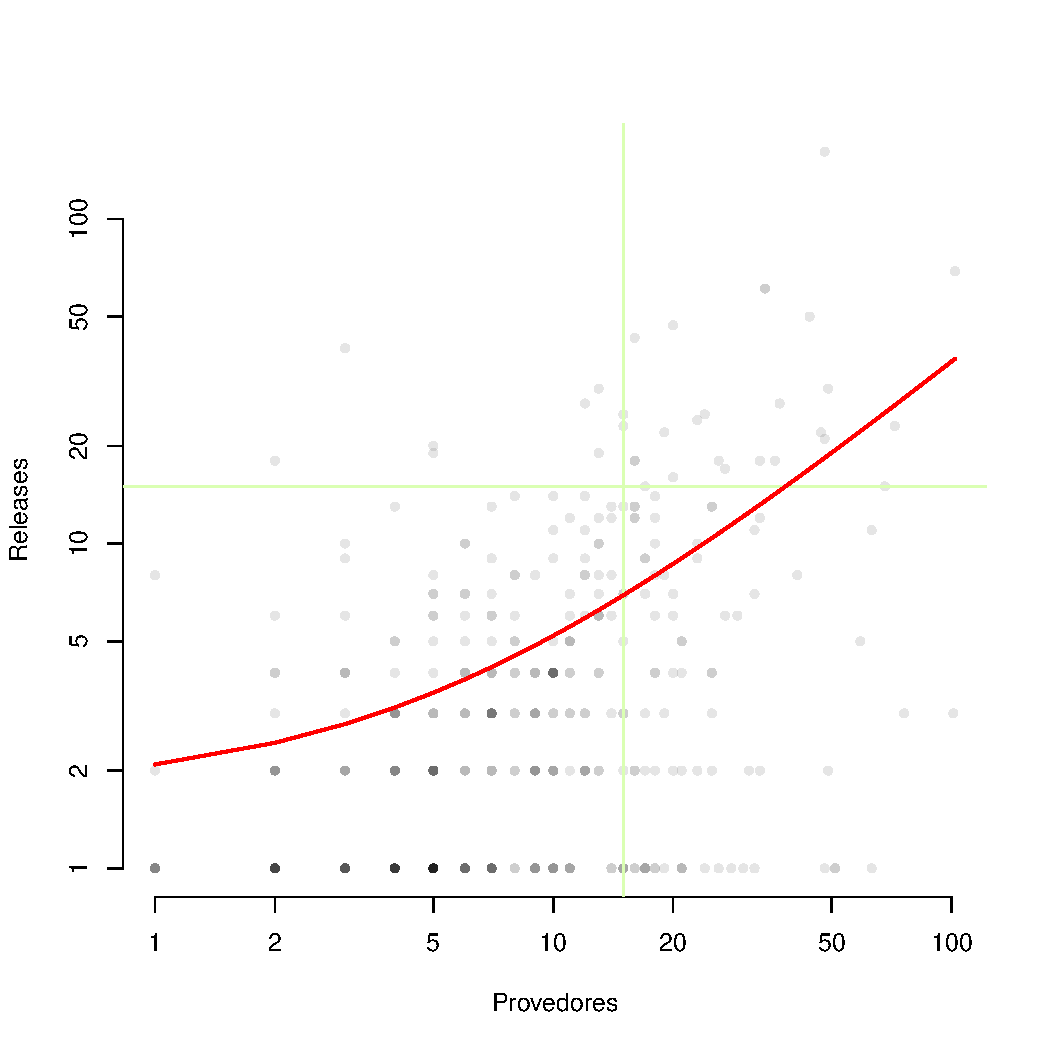
\includegraphics[scale=0.6]{figuras/correlation_release_providers.pdf}
    \caption{Correlação entre a quantidade de \textit{releases} e de provedores da amostra}
    \label{fig:correlation_release_providers}
\end{figure}{}

A análise dos clientes com \textit{breaking changes} se encontra na Figura \ref{fig:result_rq1_releases_affecteds}, que correlaciona a quantidade de provedores com a quantidade de \textit{releases} que foram executados os testes, respectivamente no eixo \textit{y} e \textit{x}. Nessa Figura, assim como na Figura anterior, estão dispersos os clientes da amostra e, em destaque, os que sofreram com \textit{breaking changes}. O tamanho dos círculos  representam a proporção de \textit{releases} dos clientes que foram impactadas, ou seja, a quantidade de \textit{releases} com os testes executados pela quantidade de \textit{releases} impactadas por \textit{breaking changes}. Assim, quanto maior os círculos vermelhos, maior o impacto das \textit{breaking changes}. Por fim, há uma regressão não-linear da relação dos provedores com as \textit{releases} dos clientes afetados com \textit{breaking changes} e uma linha vertical e uma horizontal significando a mediana das \textit{releases} e dos provedores que foram impactados por \textit{breaking changes}, respectivamente, e essas medianas valem 8 e 14, assim, dividindo o plano cartesiano em 4 quadrantes. A Figura \ref{fig:percentage_clients_bc} contém a porcentagem de clientes de cada quadrante da Figura \ref{fig:result_rq1_releases_affecteds}. Por exemplo, o quadrante superior esquerdo da Figura \ref{fig:result_rq1_releases_affecteds} contém 17.2\% dos clientes da amostra, como pode ser visto no seu respectivo eixo (\textit{Sup. esquerdo}) na Figura \ref{fig:percentage_clients_bc}, e desses 17.2\%, 10.6\% foram afetados com \textit{breaking changes}, ou seja, esses 10.6\% são a porcentagem de clientes impactados por \textit{breaking changes} nesse determinado quadrante.

\begin {figure} [h!]
   \centering
   \mbox {
        \subfigure[]{\label{fig:result_rq1_releases_affecteds} 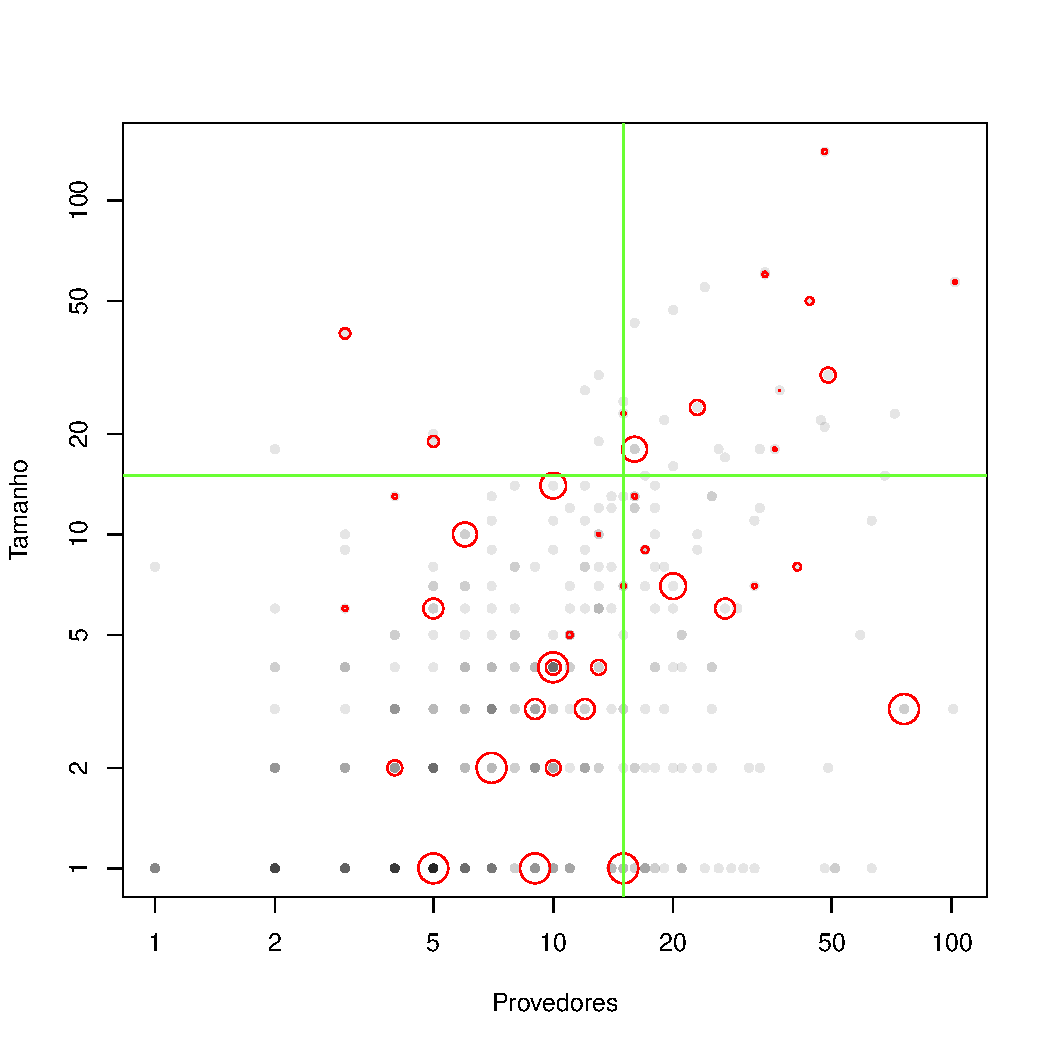
\includegraphics[scale=0.45]{figuras/result_rq1_releases_affecteds.pdf}}\quad
        \subfigure[]{\label{fig:percentage_clients_bc} 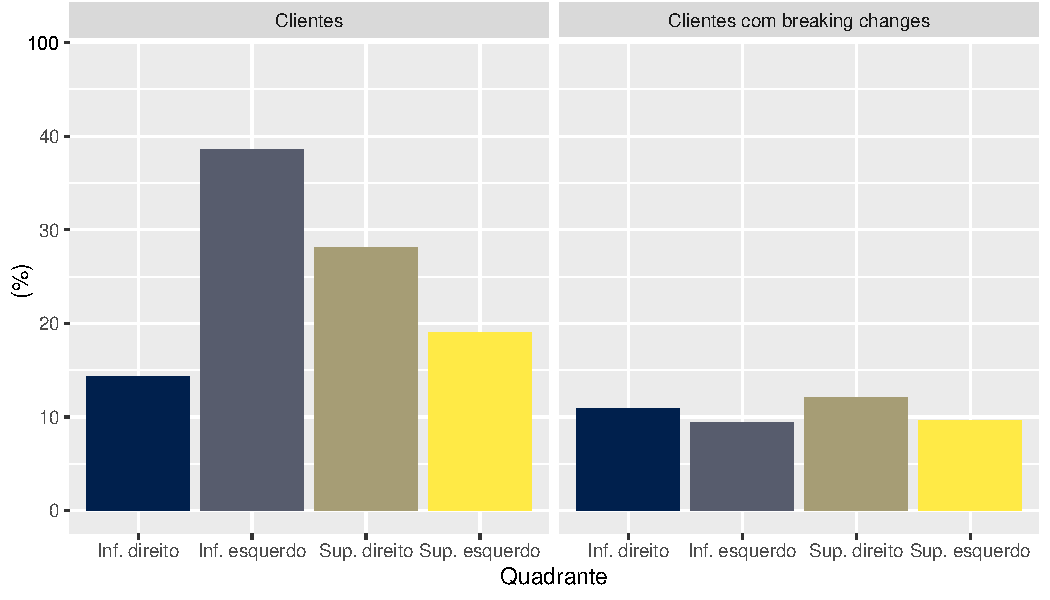
\includegraphics[scale=0.3]{figuras/percentage_clients_bc.pdf}}
    }
    \caption{(a) Dispersão das \textit{break changes} em função da quantidade de \textit{releases} e de provedores; (b) percentual de clientes de cada quadrante da Figura \ref{fig:result_rq1_releases_affecteds}}
    \label{fig:result_rq1_once_twice_three}
\end{figure}

Através da regressão não-linear da Figura \ref{fig:result_rq1_releases_affecteds}, verifica-se que a manifestação das \textit{breaking changes} está relacionada com o número de \textit{releases} executadas e com o número de provedores, uma vez que a regressão é crescente conforme a quantidade de provedores e de \textit{releases} aumentam. Mas, no quadrante em que há a maior concentração de clientes (inferior esquerdo), com 64.6\% dos clientes da amostra, há a mais baixa porcentagem de casos de \textit{breaking changes}, com um total de 5.6\% de ocorrências, mesmo sendo o quadrante com mais clientes. Neste caso, conclui-se que a manifestação de \textit{breaking changes} para clientes com um quantidade abaixo da mediana de provedores e de \textit{releases} não é comum, ou seja, os clientes com poucos provedores e poucas \textit{releases} foram os menos impactados. Ainda analisando a Figura \ref{fig:percentage_clients_bc}, é possível verificar que a manifestação de \textit{breaking changes} está fortemente relacionada com a quantidade de \textit{releases} do cliente. Essa relação está no fato de que os quadrantes com os maiores percentuais de ocorrência de \textit{breaking changes} são os quadrantes \textit{superior direito} e \textit{inferior direito}, com 30.2\% e 22.2\% de seus clientes impactados, respectivamente, e a Figura \ref{fig:result_rq1_releases_affecteds} mostra que esses dois quadrantes são os que possuem os clientes com a quantidade de \textit{releases} acima da mediana. E, como a quantidade de \textit{releases} que tiveram seus testes executados está diretamente relacionada com as atualizações dos provedores -- os testes das \textit{releases} só foram executados quando havia algum provedor que tinha publicado uma nova \textit{release} --, conclui-se que a manifestação das \textit{breaking changes} é motivada pela frequência com que os provedores publicam suas \textit{releases}. Clientes que possuem grande quantidade de provedores, mas que possuem poucas \textit{releases} com seus testes executados, não são tão impactados por \textit{breaking changes} quanto os clientes que tiveram uma grande quantidade de \textit{releases} com testes executados.

\subsubsection{Fase de desenvolvimento para a introdução das \textit{breaking changes}}

Um provedor evolui conforme os seus desenvolvedores publicam \textit{releases}, sejam essas contendo correções, melhorias ou novas funcionalidades. Durante o desenvolvimento dos provedores, os desenvolvedores tendem a ter uma visão mais clara de como evoluir seus provedores evitando \textit{breaking changes}, assim as \textit{releases} tendem a ser menos instáveis. Contudo, até mesmo provedores estáveis e com código bem desenvolvido podem introduzir \textit{breaking changes} após muito tempo de desenvolvimento, mas em um estágio avançado de desenvolvimento os provedores deveriam ser mais estáveis. Entretanto, nem sempre isso acontece. A Figura \ref{fig:providers_releases_bc} apresenta a porcentagem de cada provedor que foi desenvolvida até o surgimento da \textit{breaking change}, ou seja, em qual estágio de desenvolvimento a determinada \textit{breaking change} foi introduzida. Dessa análise foram removidos quatro provedores que introduziram \textit{breaking changes} na primeira \textit{release} e dois que introduziram \textit{breaking changes} além da data da coleta de dados, descrita na Seção \ref{sec:col_base}. Assim, foram analisados 30 provedores. \daniel{Eu não considerei os casos introduzidos na primeira release porque o provedor praticamente não foi desenvolvido ainda. Será que devo considerar esses 4 casos?}

\begin{figure}
	\centering
	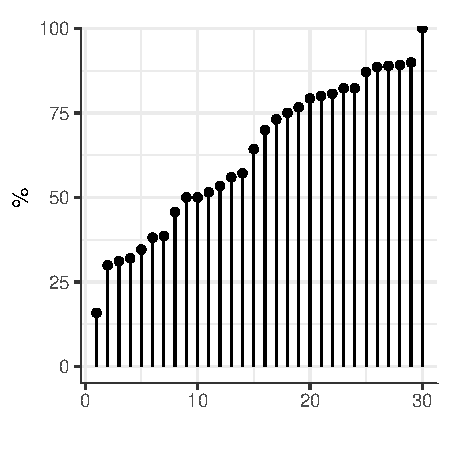
\includegraphics{figuras/providers_releases_bc.pdf}
	\caption{Fase de desenvolvimento do provedor no qual a \textit{breaking change} foi inserida}
	\label{fig:providers_releases_bc}
\end{figure}{}

Através da Figura \ref{fig:providers_releases_bc} percebe-se que as \textit{breaking changes} são mais introduzidas em um estágio avançado do provedor, uma vez que apenas 8 (26.7\%) provedores introduziram \textit{breaking changes} antes do desenvolvimento chegar a 50\%.  Isso significa que esses provedores introduziram as \textit{breaking changes} em suas primeiras \textit{releases}, e isso pode ser muito desfavorável para os provedores e pode acarretar na perca de clientes, uma vez que se os provedores possuem poucas \textit{releases}, os clientes podem não ter a opção de realizar um \textit{dowgraded} para uma \textit{release} estável dos provedores e aguardar a publicação de uma \textit{release} com a correção da \textit{breaking change} pode não ser viável e isso pode induzir o cliente a trocar de provedor.

Os provedores que introduziram \textit{breaking changes} entre os 50\% e antes dos 75\% de desenvolvimento foram 9 (30\%). Nessa fase de desenvolvimento, os provedores deveriam ser bem estáveis e não apresentar \textit{breaking changes}, uma vez que o desenvolvimento está mais avançado e os clientes podem estar usando várias interfaces dos provedores, e ter que alterar seu provedor quando se utiliza muitos recursos dele é algo muito custoso para o cliente. Entretanto, como mais da metade das \textit{releases} dos provedores já foram publicadas, o cliente pode optar em realizar um \textit{dowgraded} para uma versão estável dos provedores enquanto a correção da \textit{breaking change} não é publicada. Assim, as \textit{breaking changes} nessa fase de desenvolvimento são mais fáceis de tratar por parte do cliente.

Por fim, os provedores que introduziram \textit{breaking changes} após os 75\% de desenvolvimento foram 13 (43.3\%) provedores. Nessa fase de desenvolvimento o cliente pode facilmente realizar um \textit{dowgraded} para uma \textit{release} estável e, por ser introduzida em uma fase mais recente de desenvolvimento, o provedor pode ter alcançado vários clientes e ser motivado a consertar a \textit{breaking change} com mais rapidez.
\section{RQ2. Como os pacotes provedores introduzem \textit{breaking changes} em uma \textit{release}?}
\label{sec:qp2:results}

\subsubsection{Categorias de \textit{Breaking changes}}
Ao todo, foram 45 casos de \textit{breaking changes} distribuídas em 40 clientes. Todos esses casos foram agrupados em 8 diferentes categorias das quais se encaixavam os casos semelhantes. A Tabela \ref{tab:bc_category} apresenta cada uma dessas categorias, bem como a quantidade de pacotes e a quantidade de \textit{releases} que cada categoria atingiu.

\begin{table*}\centering
	\begin{tabular}{lrrrrr} \toprule
		\textbf{Categoria} & \multicolumn{2}{c}{Pacotes} & \phantom{ab} & \multicolumn{2}{c}{\textit{Releases}}
		\\
		\cmidrule{2-3} \cmidrule{5-6}
		& afetados & (\%) && afetadas & (\%) \\ \midrule
		Alteração de regras          & 14              & 31,11 && 67                          & 34,71 \\
		Provedores incompatíveis     & 11              & 24,44 && 37                          & 19,17 \\
		Alteração de tipo de objeto  & 7               & 15,55 && 22                          & 11,39 \\
		Objeto indefinido            & 4               & 8,88  && 25                          & 12,95 \\
		Código não-atualizado        & 3               & 6,66  && 25                          & 12,95 \\
		Código errado                & 3               & 6,66  && 11                          & 5,69  \\
		Renomeação de função         & 2               & 4,44  && 2                           & 1,03  \\
		Arquivo não encontrado       & 1               & 2,22  && 4                           & 2,07  \\ \hline
		\textbf{Total}               & \textbf{45}     &       && \textbf{193}              &       \\
		\bottomrule
	\end{tabular}
    \caption{Categorias dos casos de \textit{breaking changes}}
    \label{tab:bc_category}
\end{table*}

A seguir, encontra-se uma descrição sobre cada categoria e um exemplo de como os pacotes dessa determinada categoria foram afetados.

\begin{itemize}
    \item \textbf{Alteração de regras}: este caso foi o principal que impactou os pacotes. Essa categoria contém os casos de \textit{break change} no qual os provedores possuíam um determinado comportamento, mas alteraram algumas de suas regras/funcionalidades e impactaram os seus clientes. Não foi uma simples alteração no código, tal como uma alteração de tipo de variáveis, ou um código escrito de maneira errada, mas sim uma regra no qual o cliente tinha como sólida, foi alterada. Por exemplo, o pacote \textit{request@2.17.0} -- essa \textit{release} não existe mais no \textit{npm}, mas a alteração se manteve -- introduziu uma alteração em seu código\footnote{https://github.com/request/request/commit/d05b6ba72702c2411b4627d4d89190a5f2aba562\#diff-168726dbe96b3ce427e7fedce31bb0bcR857}, como pode ser visto na Figura \ref{fig:bc_category_change_rule_1}.

    \begin{figure}
        \centering
        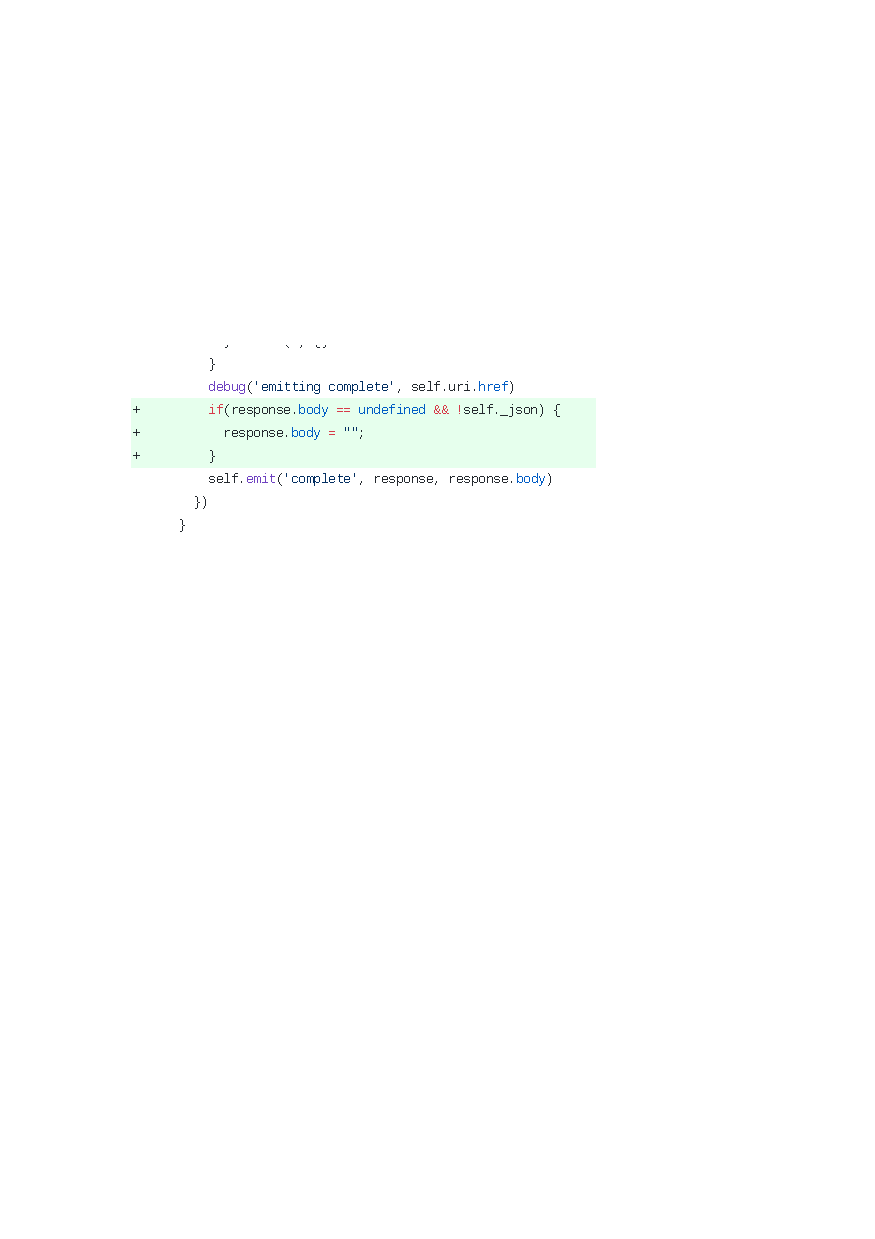
\includegraphics{figuras/bc_category_change_rule_1.pdf}
        \caption{Alteração de regra de funcionamento do \textit{request}}
        \label{fig:bc_category_change_rule_1}
    \end{figure}{}

    Nesse caso, o \textit{request} adiciona uma \textit{string} vazia ao invés de manter \textit{undefined} o corpo de uma requisição. Esse caso do \textit{request} ocorreu exatamente como foi explicado por \citeonline{Foo:2018:ESC:3236024.3275535} dizendo que os pacotes evoluem independentemente dos clientes. Essa alteração na regra do \textit{request} reflete em uma evolução do pacote, mas o cliente não esperava essa alteração e confiava que o corpo da resposta fosse retornado como \textit{undefined} em caso de erro, por isso o cliente resultou em um erro.

    \item \textbf{Provedores incompatíveis}: nessa categoria, há um provedor direto A e um provedor indireto B envolvido, o qual alterou o seu código, o que não gerou um erro, mas provocou no provedor A um comportamento inesperado, ou seja, o provedor B passou a ser incompatível com o provedor A. Nessa categoria, nenhum dos provedores contém um erro, mas sim uma incompatibilidade. Um exemplo disso ocorreu com os pacotes \textit{babel-eslint}\footnote{https://www.npmjs.com/package/babel-eslint} e \textit{escope}\footnote{https://www.npmjs.com/package/escope}, sendo o pacote \textit{escope} é um provedor indireto do \textit{babel-eslint}.

    \begin{figure}
        \centering
       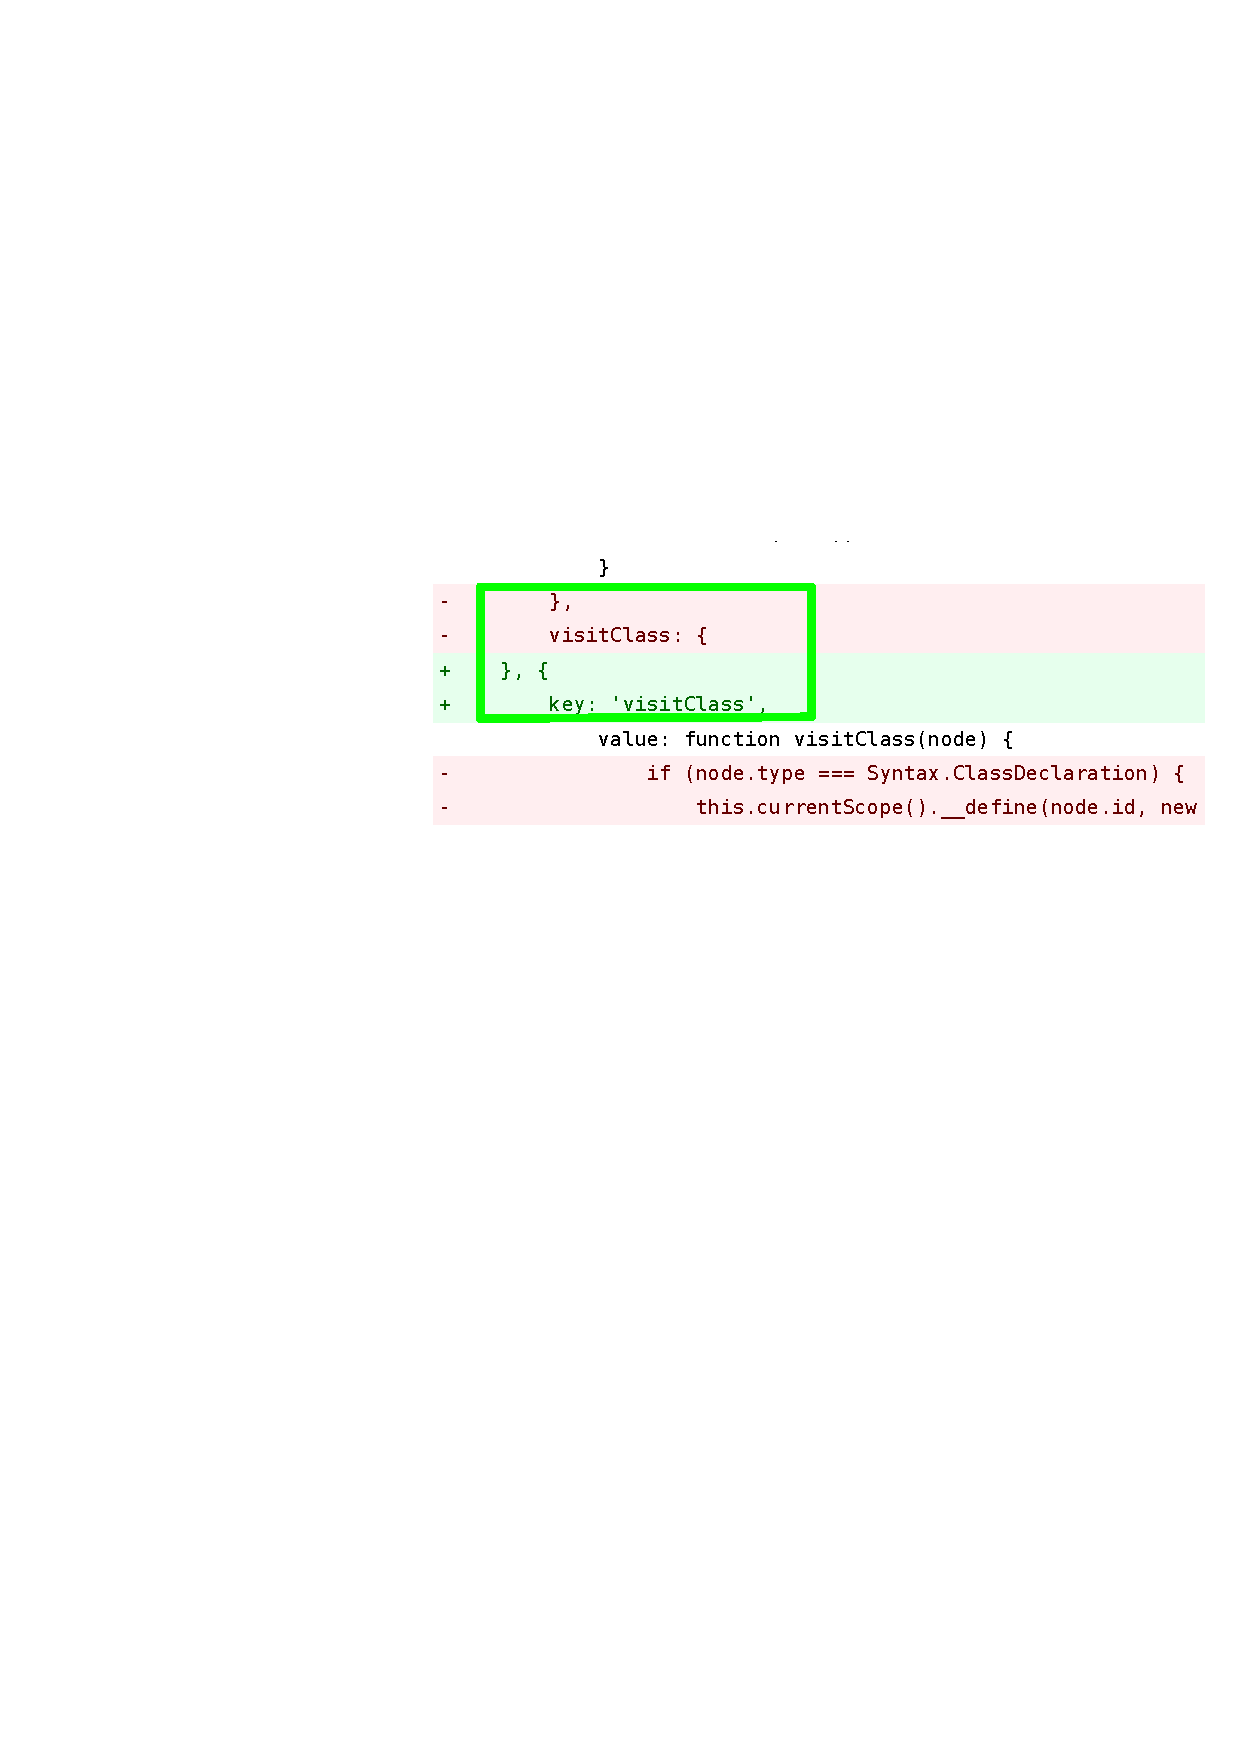
\includegraphics[scale=0.7]{figuras/bc_category_incompatibles_providers.pdf}
        \caption{Alteração de código do \textit{escope}}
        \label{fig:bc_category_incompatibles_providers}
    \end{figure}{}

    A \textit{release escope@3.4} realizou uma alteração no seu código, de acordo com a Figura \ref{fig:bc_category_incompatibles_providers}, mas que não reflete em um erro. Essa alteração impactou diretamente o pacote \textit{babel-eslint}, mesmo o pacote \textit{escope} não sendo um provedor direto do \textit{babel-eslint} e não ter introduzido um erro\footnote{https://github.com/estools/escope/issues/99\#issuecomment-178151491}. Com isso, há uma incompatibilidade entre os provedores e essa incompatibilidade precisou ser corrigida pelo \textit{babel-eslint} e não pelo \textit{escope}. Essa foi a \textit{breaking change} que mais surgiu na análise manual pois, dos 45 casos, 6 (13.3\%) refletiam essa incompatibilidade, uma vez que o \textit{babel-eslint} é provedor direto de 5.8\% de todo o conjunto de dados.

    \item \textbf{Alteração de tipo de objeto}: essa é uma categoria de \textit{break changes} facilmente detectável em linguagens fortemente tipadas, mas no \textit{Javascript} representam um tipo de \textit{break change} que, por muitas vezes, pode nem afetar o código do cliente. Mas, neste trabalho, foram detectados 7 (15.5\%) de casos nos quais os provedores alteraram o tipo de alguma variável.

    \begin{figure}
        \centering
        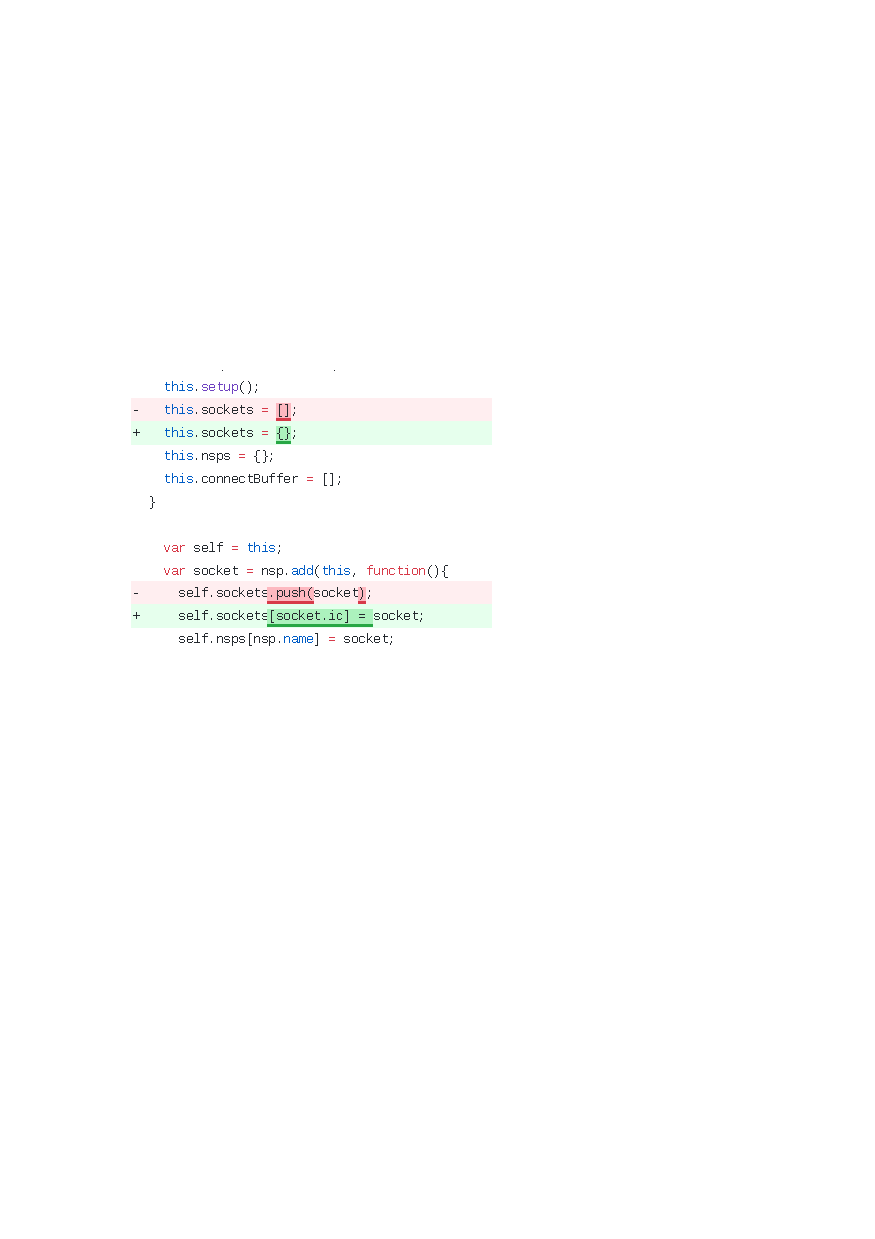
\includegraphics[scale=0.9]{figuras/bc_category_change_type.pdf}
        \caption{Alteração de um tipo \textit{array} para \textit{object}}
        \label{fig:bc_category_change_type}
    \end{figure}{}

    Na Figura \ref{fig:bc_category_change_type} o provedor \textit{socket.io}\footnote{https://www.npmjs.com/package/socket.io} alterou alguns \textit{arrays} para \textit{object}\footnote{https://github.com/socketio/socket.io/commit/b73d9bea4efb48277eee685763026ff2df5a79ab}. Anteriormente, os clientes iteravam nesses \textit{arrays}, mas após essa alteração, os clientes foram afetados.

    \item \textbf{Objeto indefinido}: por vezes, os códigos podem estar todos corretos, mas então o provedor tenta acessar uma variável que não existe. Esta categoria de \textit{break change} representa os casos no qual os provedores tentaram obter acesso à alguma variável/objeto, mas que não existiam. Esses erros são os que facilmente podem ser consertados/evitados apenas adicionando o código da Listagem \ref{cod:undefined_object}:

    \begin{lstlisting}[style=bash, label=cod:undefined_object]
    this.var = this.var || {};
    \end{lstlisting}

    Esse tipo de erro surgiu no pacote \textit{ember-cli-htmlbars-inline-precompile}\footnote{https://www.npmjs.com/package/ember-cli-htmlbars-inline-precompile}, no qual o desenvolvedor tenta acessar uma variável que não estava disponível. Mas, assim como o desenvolvedor já havia feito com as demais variáveis da Figura \ref{fig:bc_category_undefined_object}, uma simples alteração no código foi o suficiente\footnote{https://github.com/ember-cli/ember-cli-htmlbars-inline-precompile/pull/5/commits/b3faf959fcea8e5b928f4fa28bf6572534968d81\#diff-168726dbe96b3ce427e7fedce31bb0bcR13}.

    \begin{figure}
        \centering
        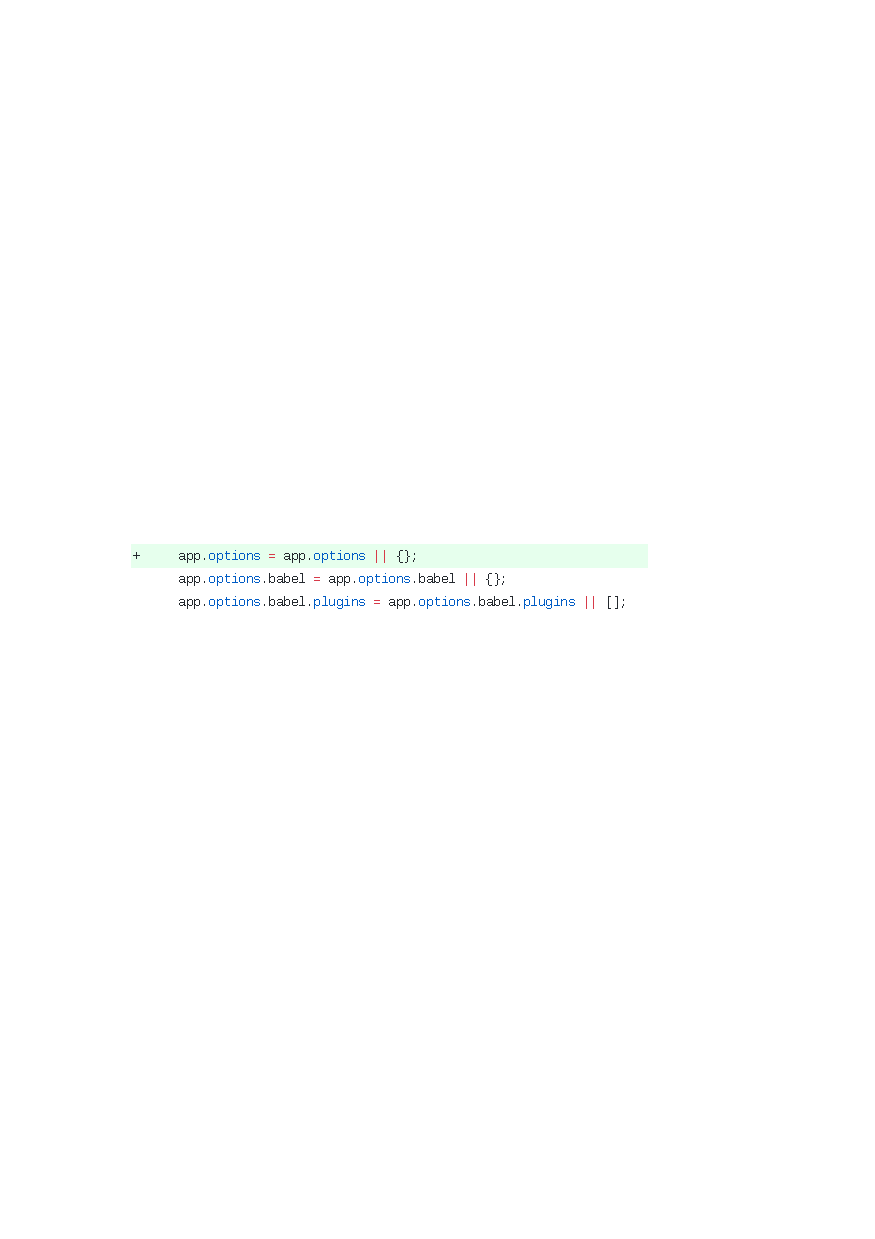
\includegraphics{figuras/bc_category_undefined_object.pdf}
        \caption{Correção do erro de objeto indefinido}
        \label{fig:bc_category_undefined_object}
    \end{figure}{}

    \item \textbf{Código errado}: este caso de \textit{breaking change} ocorreu quando o provedor escreveu um código semanticamente incorreto, gerando um erro na sua execução e afetando o cliente. Em linguagens compilada, esse tipo de erro seria facilmente identificado pelo compilador em tempo de compilação. Foi exatamente isso que a dependência front-matter@0.2.0\footnote{https://github.com/jxson/front-matter/commit/f16fc01d88ff7b93f65ebfbdc957fd66cd5a2002\#diff-168726dbe96b3ce427e7fedce31bb0bcL4} fez. Ao alterar o seu código, o desenvolvedor escreveu duas vezes a mesma variável, como pode ser visto na Figura \ref{fig:bc_category_wrong_code}. Assim como os erros do tipo \textit{undefined object}, os erros dessa categoria são facilmente corrigidos.

    \begin{figure}
        \centering
        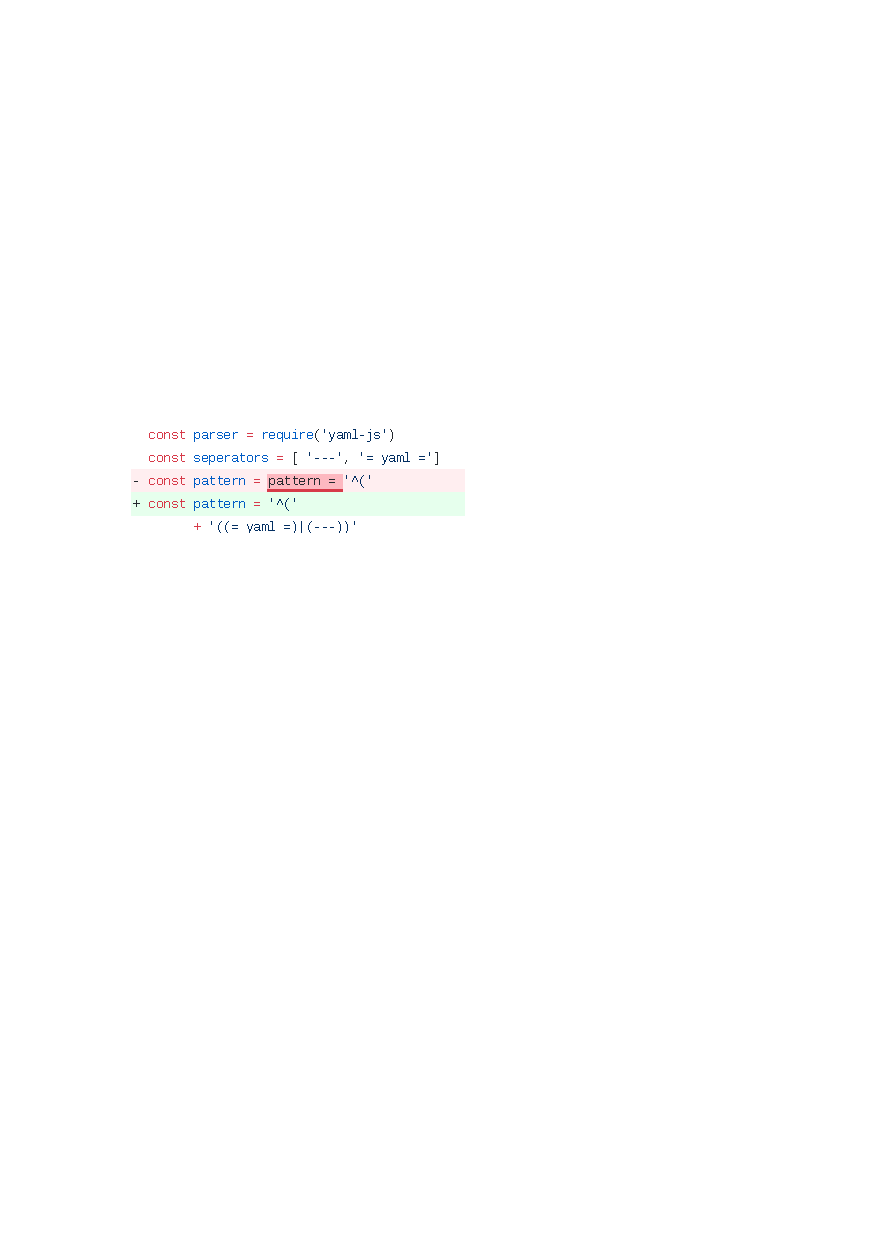
\includegraphics[scale=1.2]{figuras/bc_category_wrong_code.pdf}
        \caption{Código semanticamente incorreto}
        \label{fig:bc_category_wrong_code}
    \end{figure}{}

    \item \textbf{Renomeação de função}: as \textit{breaking changes} relacionadas à esta categoria foram facilmente detectáveis. Quando a mensagem de erro do \textit{node.js} era exibida como \textit{TypeError: var is not a function}, com pouca investigação já era possível saber que uma determinada função não estava mais disponível, ou seja, havia sido removida ou renomeada. E foi exatamente esta \textit{breaking change} que o provedor redis@2.6.0-1\footnote{https://github.com/NodeRedis/node_redis/commit/861749f4d6be28ee861096765e7176dc988024f6\#diff-168726dbe96b3ce427e7fedce31bb0bcL763} introduziu, conforme a \ref{fig:bc_category_renamed_function}.

    \begin{figure}
        \centering
        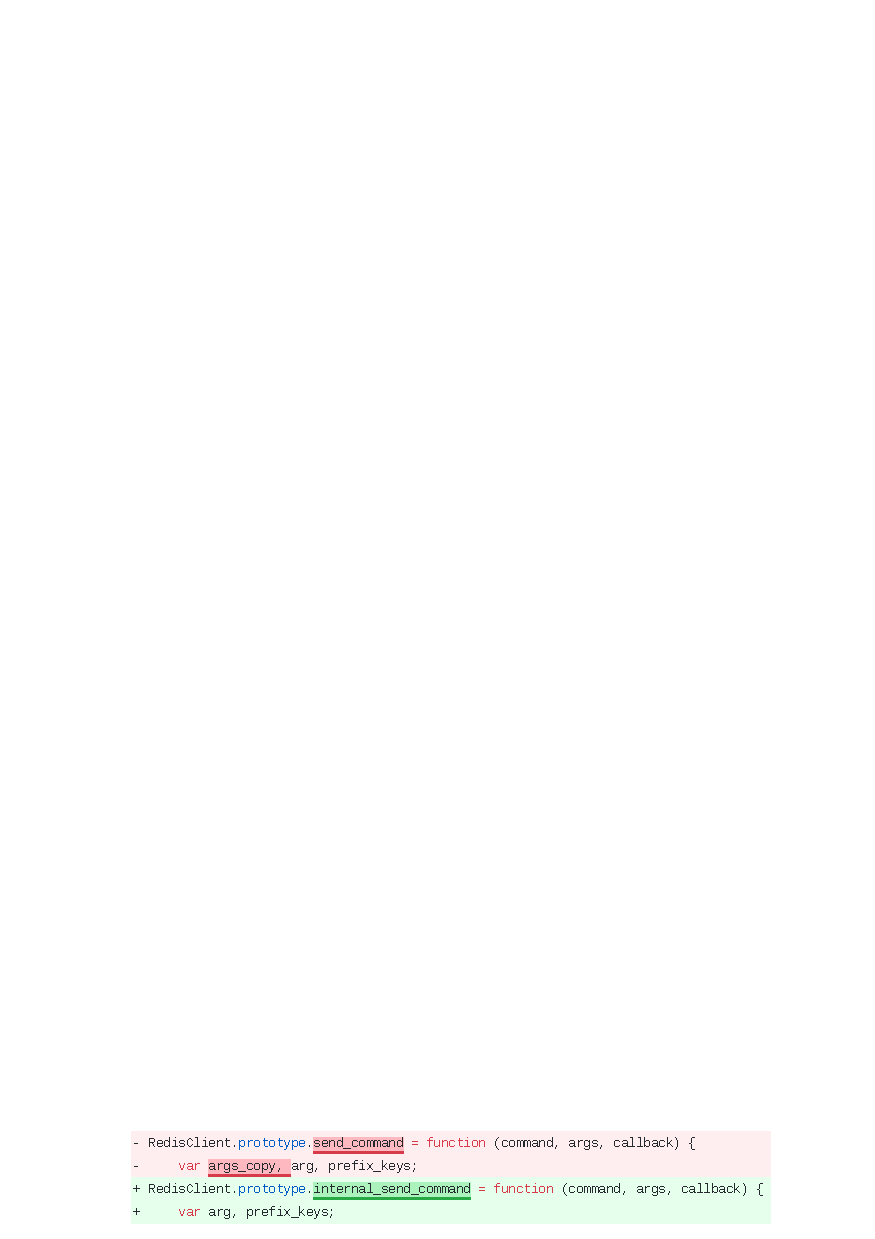
\includegraphics{figuras/bc_category_renamed_function.pdf}
        \caption{Alteração do nome de função}
        \label{fig:bc_category_renamed_function}
    \end{figure}{}

    \item \textbf{Arquivo não encontrado}: os casos de \textit{breaking change} relacionados à esta categoria são aqueles no qual o desenvolvedor realiza um acesso a um arquivo, mas esse não existe. O arquivo requerido pode não existir ou não estar disponível, uma vez que, referenciado no arquivo \textit{.npmignore} -- arquivo utilizado pelo \textit{npm} para ignorar arquivos durante o processo de publicação --, o arquivo existe mas não está disponível, mas também o arquivo pode não existir. Entretanto, o único caso de arquivo não encontrado ocorreu pois o arquivo \textit{index.js} estava indisponível. O provedor \textit{esprima-extract-comments}\footnote{https://www.npmjs.com/package/esprima-extract-comments} utilizava como provedor um \textit{fork} do pacote \textit{esprima}\footnote{https://github.com/ariya/esprima/} e o referenciava em seu  \textit{package.json} para ser descarregado diretamente do \textit{Github}\footnote{https://github.com/jonschlinkert/esprima-extract-comments/blob/6b65a0f52f85bc6fa830d44e352ec3da9e9ef620/package.json\#L47}. Entretanto, o \textit{index.js} desse \textit{fork}, foi referenciado no \textit{.gitignore} e não estava disponível quando o \textit{npm} descarregou o pacote diretamente do \textit{Github}, mas o arquivo estava disponível se esse clone do pacote \textit{esprima} fosse descarregado diretamente do \textit{npm}.

\end{itemize}{}

\subsubsection{Níveis do Versionamento Semântico nos quais as \textit{breaking changes} são introduzidas}
O Versionamento Semântico foi desenvolvido para padronizar o versionamento de \textit{softwares} e facilitar para o cliente decidir quais as novas atualizações que ele deseja receber de um provedor. Entretanto, por vezes os desenvolvedores realizam o versionamento erroneamente, o que pode impactar os clientes negativamente, principalmente quando há \textit{breaking changes} em \textit{releases não-major}. Foi exatamente isso que ocorreu. Dos 45 casos de \textit{breaking changes}, 26 casos foram introduzidos no nível \textit{minor}; 16 casos, \textit{patch}; 2 casos, \textit{major}; e 1 caso foi introduzido em uma \textit{pre-release}, como pode ser visto na Tabela \ref{tab:semver_levels}. Os casos de \textit{breaking changes} que foram introduzidos em \textit{releases major} ou \textit{pre-releases} são \textit{breaking changes} devidamente introduzidas, mas um provedor direto não tratou essas \textit{breaking changes} introduzidas por um provedor indireto, o que acarretou na manifestação da \textit{breaking change} no cliente.

\begin{table}[]
\centering
\begin{tabular}{lr}
\toprule
\textbf{Níveis}      & \textbf{\%} \\ \hline
\textit{Major}       & 4.44\%      \\
\textit{Minor}       & 57.78\%     \\
\textit{Patch}       & 35.56\%     \\
\textit{Pré-release} & 2.22\%      \\ \bottomrule
\end{tabular}
\caption{Porcentagem de \textit{breaking changes} em cada um dos níveis do Versionamento Semântico}
\label{tab:semver_levels}
\end{table}

Mais da metade das \textit{breaking changes} foram introduzidas em \textit{releases minor} (57.78\%). Isso significa que, de acordo com as regras do Versionamento Semântico, os provedores tinham o interesse de publicar novas funcionalidades que mantivessem a compatibilidade com as \textit{releases} anteriores, mas essas novas funcionalidades resultaram em erros nos clientes. Entretanto, essas novas funcionalidades introduzidas pelos provedores podem caracterizar realmente casos de \textit{breaking changes}, no qual os provedores precisaram consertar o código, mas também podem ser apenas novas funcionalidades na qual os clientes precisaram se adequar, pois as \textit{breaking changes} foram causadas não por um erro nos provedores, mas sim por um erro de utilização nos clientes.
\daniel{Será que é viável retomar o exemplo a seguir?}
Foi exatamente isso que ocorreu no exemplo da Figura \ref{fig:bc_category_change_rule_1} em Categorias de \textit{Breaking Changes} na Seção \ref{sec:qp2:results}, na categoria \textit{Alterações de regras}, na qual é possível ver que o provedor desenvolveu uma nova funcionalidade que não continha um erro, mas acabou introduzindo uma \textit{breaking change} no cliente, e essa \textit{breaking change} não foi corrigida pelo provedor, uma vez que essa alteração apenas refletia uma evolução do provedor. Assim sendo, para o cliente o código se trata de uma \textit{breaking change}, mas para o provedor, não.

Para verificar se as \textit{breaking changes} introduzidas em \textit{releases minor} refletem em \textit{breaking changes} no qual os provedores consertaram seu código, ou se refletem em uma nova funcionalidade que os clientes tiveram que se adequar, foi analisado para cada caso de \textit{breaking change} introduzida em \textit{releases minor}, qual pacote que consertou a \textit{breaking change} -- cliente ou provedor -- e qual foi o nível do Versionamento Semântico na qual a \textit{release} que contém a correção foi publicada. Esses dados estão na Figura \ref{fig:semver_fixed}, na qual, dos 26 casos de \textit{breaking changes} introduzidas em \textit{releases minor}, 4 casos foram consertados pelos provedores; 20 pelos clientes; e 2 casos não foram consertados por ambos.

\begin{figure}
    \centering
    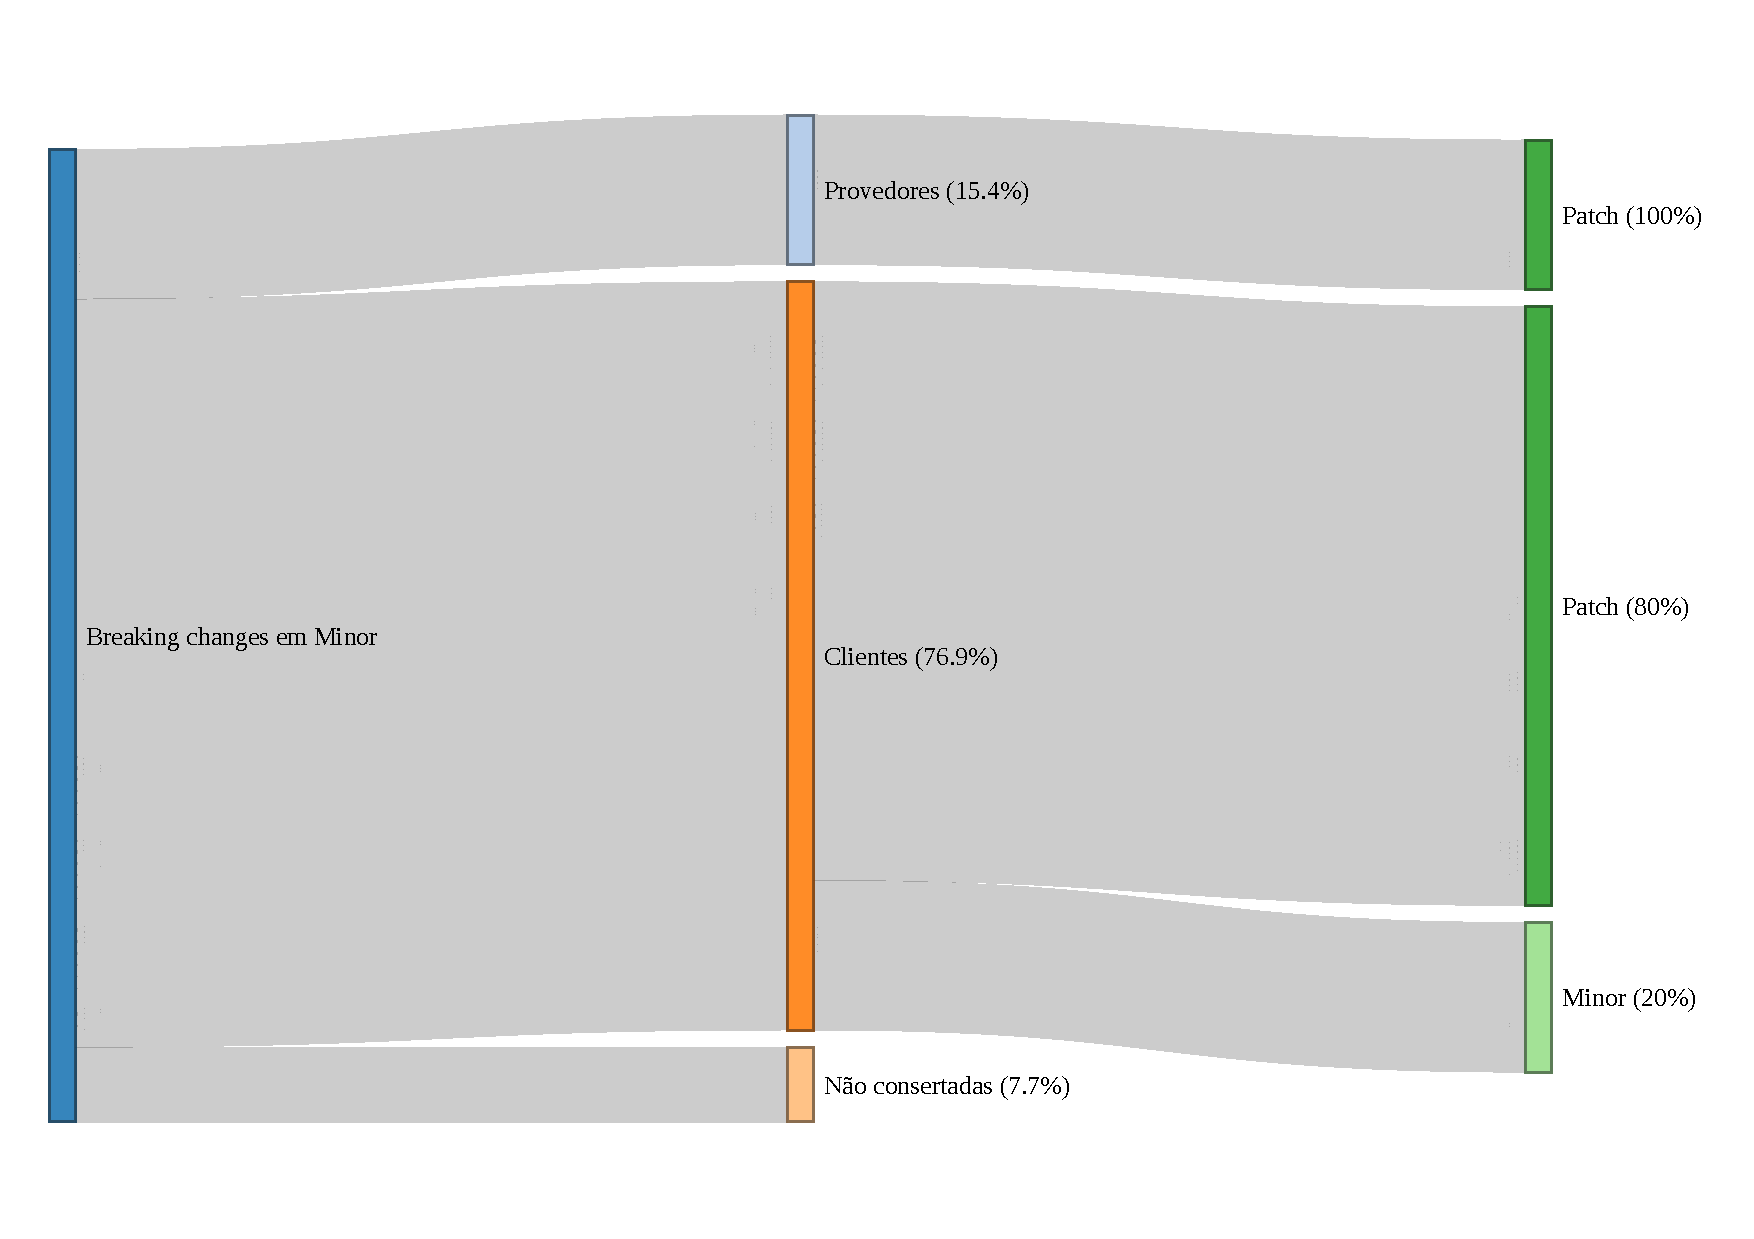
\includegraphics[scale=0.5]{figuras/semver_fixed.pdf}
    \caption{\textit{Breaking changes} consertadas pelo provedor e pelo cliente e os níveis do Versionamento Semântico das \textit{releases} com a correção}
    \label{fig:semver_fixed}
\end{figure}{}

Na Figura \ref{fig:semver_fixed}, é possível verificar que mais da metade dos casos de \textit{breaking changes} que foram introduzidas em \textit{releases minor} (76.9\%) foram consertados pelos clientes. Isso significa que os provedores introduziram novas funcionalidades, que não refletiam em um erro, mas que causaram um comportamento inesperado nos clientes, e foram os clientes os responsáveis por consertar seus códigos para que a nova \textit{release} dos provedores, mesmo sendo retro-compatível, pudesse executar com sucesso. Assim, a maior parte das \textit{breaking changes} não ocorreram porque os provedores introduz um erro em seus códigos e esse erro é cascateado para os clientes, mas sim porque os clientes utilizam o provedor de maneira errada e necessitam consertar o seu código para se adequar às novas funcionalidades introduzidas pelos provedores. Isso é perceptível, pois quando os cliente consertam os seus códigos e os publicam, em 80\% dos casos são publicados em uma \textit{release patch}, ou seja, de acordo com as regras do Versionamento Semântico, os clientes estão consertando algum determinado erro, que pode ser o modo como os clientes utilizam os provedores.

Quando os provedores consertam as \textit{breaking changes}, em 100\% dos casos essa correção é publicada em uma \textit{release patch}, que de acordo com as regras do Versionamento Semântico, são alterações no código que os provedores tinha a intenção de consertar algum determinado erro. Assim, pode-se afirmar que todos os 15.4\% dos casos de \textit{breaking changes} em \textit{releases minor} são realmente \textit{breaking changes} que deveriam ter sido publicadas em \textit{releases major}, mas que por algum motivo, os provedores introduziram em \textit{releases minor} e os clientes foram impactados por essas \textit{breaking changes}.

\subsubsection{Relação entre as categorias das \textit{breaking changes} com os níveis do Versionamento Semântico nos quais foram introduzidas}


Quando o provedor não sabe em qual nível do Versionamento Semântico uma determinada alteração deve ser introduzida, ou quando uma \textit{breaking change} é introduzida acidentalmente, o cliente pode ser impactado pela \textit{breaking change} introduzida  errôneamente em qualquer um dos níveis \textit{minor} ou \textit{patch} do Versionamento Semântico. No geral, as \textit{breaking changes} de uma determinada categoria seguem um padrão de versionamento. A Figura \ref{fig:semver_types} apresenta os casos de \textit{breaking changes} por categoria que foram inseridas em cada um dos níveis do Versionamento Semântico, sendo que os dados de cada categoria foram normalizados. \daniel{foi normalizado para ficar em porcentagem}

\begin{figure}[!h]
	\centering
	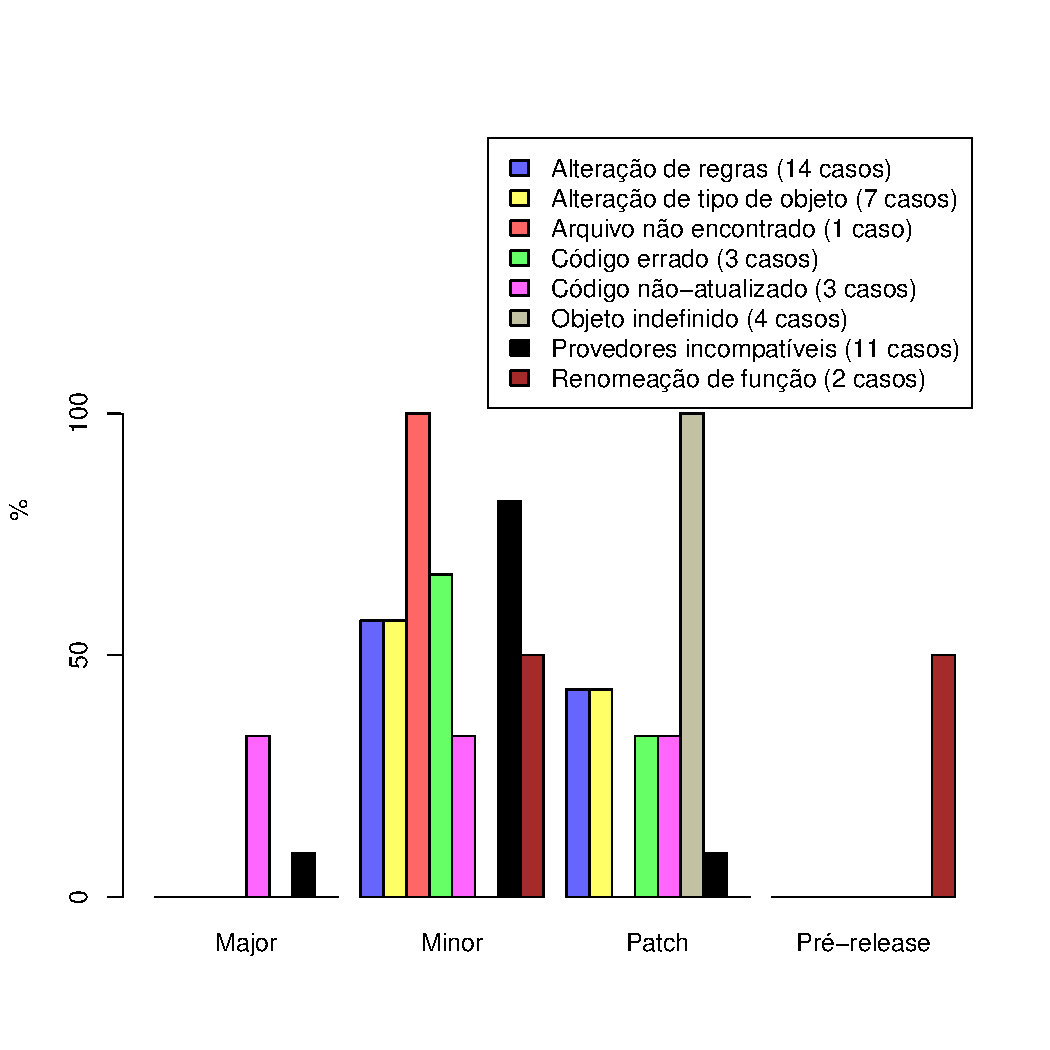
\includegraphics[scale=0.65]{figuras/semver_types.pdf}
	\caption{Os níveis do Versionamento Semântico nos quais as categorias de \textit{breaking changes} foram introduzidas}
	\label{fig:semver_types}
\end{figure}{}

As \textit{breaking changes} introduzidas nos níveis \textit{major} e \textit{pre-release} são \textit{breaking changes} que foram devidamente introduzidas por um provedor indireto, mas um provedor direto aceitou essas \textit{breaking changes}, através de seu \textit{range semver}, e  não alterou o seu código para se adaptar com as \textit{breaking changes}, fazendo com que os clientes fossem impactados por essas \textit{breaking changes}. E as \textit{breaking changes} introduzidas no nível \textit{major} são das categorias \textit{Código não-atualizado} e \textit{Provedores incompatíveis}, que são duas categorias nas quais envolve um provedor direto e um indireto. Ainda sobre essas duas categorias, há casos de \textit{breaking changes} que foram introduzidas tanto em \textit{releases minor} quando em \textit{patch} e, predominantemente,  as \textit{breaking changes} da categoria \textit{Provedores incompatíveis} foram introduzidas em \textit{releases Minor}, ou seja, dois provedores  podem se tornar incompatíveis entre sí após um deles introduzir alterações retro-compatíveis, mas que impacte o outro provedor, fazendo com que o cliente seja impactado por uma \textit{breaking change}.

Duas categorias que tiveram a mesma porcentagem foram a \textit{Alteração de regras} e a \textit{Alteração de tipo de objeto}, que tiveram 60\% e 40\% de seus casos introduzidos em níveis \textit{minor} e \textit{patch}, respectivamente. Os provedores dessas duas categorias introduziram algumas alterações/melhorias em seus códigos que impactaram os clientes com \textit{breaking changes}. Por serem majoritariamente introduzidas em \textit{releases minor}, os provedores tinha a intenção de implementar novas funcionalidades retro-compatíveis ou melhorar as funcionalidades existentes, mas alteraram as funcionalidades que os clientes previamente utilizavam, assim introduzindo uma \textit{breaking change}. Dessa maneira, alguns alterações em funcionalidades já existentes com a intenção de melhora-las deveriam ter sido introduzidas em \textit{releases major}, uma vez que ao invés de melhorar as funcionalidades, os provedores alteraram essas funcionalidades, mostrando que por vezes algumas alterações tornam-se difíceis de serem identificadas, por parte do desenvolvedor, em qual nível do Versionamento Semântico elas devem ser introduzidas.

\section{RQ3. Como os pacotes clientes se recuperam das \textit{breaking changes}?}


\subsubsection{Os clientes que se recuperaram das \textit{breaking changes}}
Quando um provedor introduz uma \textit{breaking change}, o cliente tem três opções para se recuperar: alterar o seu código para que execute mesmo com a \textit{breaking change}; aguardar o provedor corrigir o erro e, logo após, uma pratica comum é alterar a versão aceita do provedor no \textit{package.json}; ou regredir a versão do provedor no \textit{package.json} para utilizar uma que não contenha \textit{breaking changes}. Entretanto, a questão é que, por vezes, os clientes realmente se recuperam das \textit{breaking changes} sem a intervenção dos provedores. Do total de 45 casos de \textit{breaking changes} 30 dos casos foram corrigidos pelos clientes contra 12 dos casos que foram corrigidos pelos provedores  e 3 casos não foram corrigidos por ambos.

A Tabela \ref{tab:fix} apresenta a porcentagem das correções das \textit{breaking changes} pelos provedores e pelos clientes e a mediana do tempo gasto por cada um para que as \textit{breaking changes} fossem corrigidas. Os dias que os provedores gastam para corrigir as \textit{breaking changes} são maiores do que os gastos pelos clientes, uma vez que o provedor precisa ser alertado pelos clientes, análisar o caso, alterar o código, revisar as alterações e publicá-las. E muitas vezes, quando já está sendo preparada uma nova \textit{release}, os provedores podem corrigir a \textit{breaking change} mas publicá-las somente quando a proxima \textit{release} estiver pronta. Em contra partida, os clientes não precisam de todas essas etapas para se recuperar de uma \textit{breaking change}, uma vez que, eles podem simplesmente retroceder a versão do provedor no \textit{package.json} para uma em que não há \textit{breaking changes} e esperar que o mesmo publique uma \textit{release} com a correção. De todos os 30 casos de \textit{breaking changes} nos quais os clientes que corrigiram, em 20 casos foi alterada a versão do provedor no \textit{package.json} para uma versão anterior na qual não havia \textit{breaking changes} -- foi realizado um \textit{downgraded} na versão do provedor --, e a mediana do tempo gasto para os clientes corrigirem a \textit{breaking change} com a alteração da versão do provedor é, também, de 4 dias. Entretanto, mesmo alguns casos no qual o provedor corrigiu o erro, ainda em dois casos os clientes realizaram o \textit{downgraded} do provedor.

\begin{table}[!h]
\centering
	\begin{tabular}{|l|l|l|l|}
		\hline
		\centering
		& Provedor    & Cliente     & Não corrigido                             \\ \hline
		Corrigiu           & 12 (26.7\%) & 30 (66.7\%) & 3 (6.6\%)    \\ \hline
		\textit{Dowgraded} & 2  (4.4\%)  & 20 (44.4\%) & -            \\ \hline
		Dias (mediana)     & 35          & 4           & -            \\ \hline
	\end{tabular}
	\caption{Pacote que corrigiu a \textit{breaking change}, os \textit{downgrade} e a mediana do tempo gasto para ser corrigida}
	\label{tab:fix}
\end{table}
